\documentclass[12pt]{article}
\usepackage[T1]{fontenc}
\usepackage[T1]{polski}
\usepackage[utf8]{inputenc}
\newcommand{\BibTeX}{{\sc Bib}\TeX} 
\usepackage{graphicx}
\usepackage{amsfonts}
\usepackage{amsmath}
\usepackage{latexsym}
\usepackage{float}

\setlength{\textheight}{21cm}

\title{{\bf Zadanie nr 1 - Generacja sygnału i szumu}\linebreak
Cyfrowe Przetwarzanie Sygnałów}
\author{Dawid Jakubik, 224307 \and Hubert Gawłowski, 224298}
\date{08.04.2021}

\begin{document}
\clearpage\maketitle
\thispagestyle{empty}
\newpage
\setcounter{page}{1}
\section{Cel zadania}

Celem zadania było zapoznanie się z własnościami różnych sygnałów oraz poznanie i zastosowanie podstawowych działań na sygnałach. W wyniku zadania powstała aplikacja w technologii Java, która rysuje wykresy przebiegu oraz histogramy dla poszczególnych sygnałów oraz dla sygnałów powstałych w wyniku działań na dwóch sygnałach. Oblicza ona i pokazuje wartości dla sygnałów, a także zezwala za zapis i odczyt sygnału do/z pliku.

\section{Wstęp teoretyczny}

Sygnały użyte w zadaniu generowane są na podstawie wzorów znajdujących się w instrukcji do zadania \cite{instrukcja}. W instrukcji \cite{instrukcja} znajdują się także wzory użyte w celu obliczenia parametrów funkcji, czyli wartości średniej, bezwzględnej wartości średniej, wariancji, mocy średniej oraz wartości skutecznej. Aby przedstawić sygnały na wykresie, zostały one poddane próbkowaniu, czyli operacji w wyniku której powstał zbiór punktów, które po połączeniu utworzyły odpowiedni wykres.


\section{Eksperymenty i wyniki}

%%%%%%%%%%%%%%%%%%%%%%%%%%%%%%%%%%%%%%%%%%%%%%%%%%%%%%%%%%%%%%%%%%%%%%%%%%%%%%%%%%%%%%%%%%%%%%%%%%%%%%%%%%%%%%%%%
% PODROZDZIA£ PT. EKSPERYMENT NR 1 
%%%%%%%%%%%%%%%%%%%%%%%%%%%%%%%%%%%%%%%%%%%%%%%%%%%%%%%%%%%%%%%%%%%%%%%%%%%%%%%%%%%%%%%%%%%%%%%%%%%%%%%%%%%%%%%%%

\subsection{Eksperyment nr 1 : Szum impulsowy}

Celem eksperymentu było wygenerowanie szumu impulsowego. Jest to sygnał dyskretny, którego amplituda przyjmuje dwie wartości, wartość 0 oraz wartość A różną od zera.

\subsubsection{Założenia}
Wartości parametrów, jakie zostały wprowadzone do wygenerowania sygnału:
\begin{itemize}
    \item Amplituda = 4
    \item Czas początkowy = 0s
    \item Czas trwania sygnału = 5s
    \item Częstotliwość = 5Hz
    \item Prawdopodobieństwo = 50%
\end{itemize}
\subsubsection{Przebieg}
Wygenerowany został następujący sygnał:
\begin{figure}[H]
    \centering
    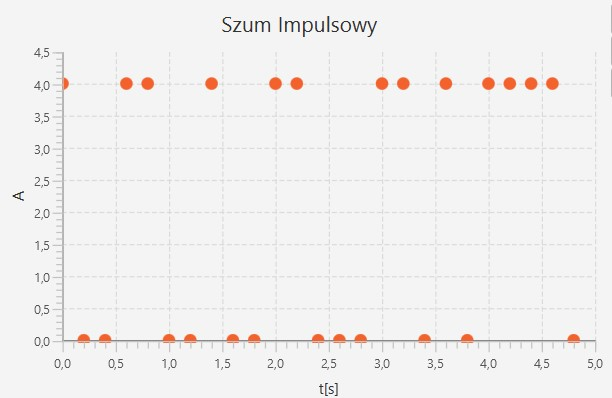
\includegraphics{cps_szum_impulsowy_sygnal.jpg}
    \caption{Wykres szumu impulsowego dla parametrów:  A=4, t1=0s, d=5s, f=5Hz, p=0.5}
    \label{wykres dla eksperymentu 1}
\end{figure}

Histogram do wygenerowanego sygnału prezentuje się następująco:
\begin{figure}[H]
    \centering
    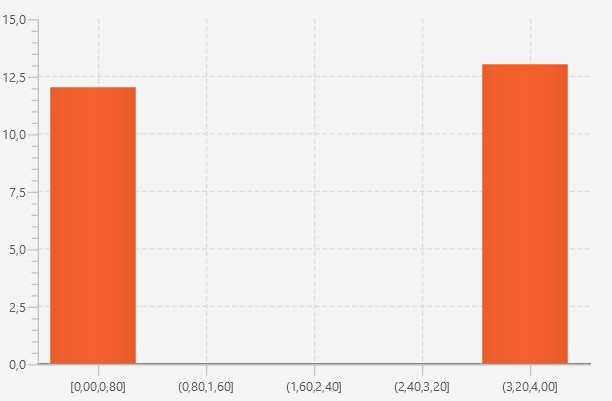
\includegraphics{cps_szum_impulsowy_histogram.jpg}
    \caption{Histogram dla szumu impulsowego o parametrach:  A=4, t1=0s, d=5s, f=5Hz, p=0.5}
    \label{histogram dla eksperymentu 1}
\end{figure}

\newpage

\subsubsection{Rezultat}
Obliczone parametry dla szumu impulsowego:
\begin{figure}[H]
    \centering
    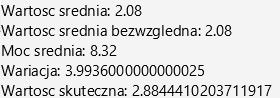
\includegraphics{cps_szum_impulsowy_wartosci.jpg}
    \caption{Obliczone wartości dla szumu impulsowego o parametrach:  A=4, t1=0s, d=5s, f=5Hz, p=0.5 }
    \label{Wartości dla eksperymentu 1}
\end{figure}


%%%%%%%%%%%%%%%%%%%%%%%%%%%%%%%%%%%%%%%%%%%%%%%%%%%%%%%%%%%%%%%%%%%%%%%%%%%%%%%%%%%%%%%%%%%%%%%%%%%%%%%%%%%%%%%%%

%%%%%%%%%%%%%%%%%%%%%%%%%%%%%%%%%%%%%%%%%%%%%%%%%%%%%%%%%%%%%%%%%%%%%%%%%%%%%%%%%%%%%%%%%%%%%%%%%%%%%%%%%%%%%%%%%

\newpage
\subsection{Eksperyment nr 2 : Szum o rozkładzie jednostajnym}

Eksperyment nr 2 polegał na wygenerowaniu szumu o rozkładzie jednostajnym. Jest to szum dla którego amplitudy są losowo wybierane z jednakowym prawdopodobieństwem z przedziału $<-A_{max},A_{max}>$.

\subsubsection{Założenia}

W eksperymencie szum wygenerowany został dla następujących parametrów:
\begin{itemize}
    \item Amplituda: 1
    \item Czas początkowy: 0s
    \item Czas trwania sygnału: 1s
\end{itemize}

\subsubsection{Przebieg}
Wygenerowany sygnał prezentuje się następująco:

\begin{figure}[H]
    \centering
    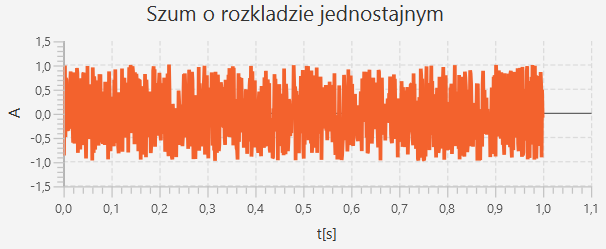
\includegraphics{cps_szum_o_rozkladzie_jednostajnym_syg.png}
    \caption{Wykres szumu o rozkładzie jednostajnym dla parametrów:  A=1, t1=0s, d=1s}
    \label{wykres dla eksperymentu 2}
\end{figure}
\newpage
Histogram dla powyższego szumu prezentuje się następująco:

\begin{figure}[H]
    \centering
    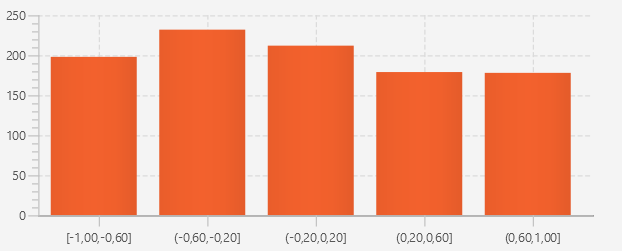
\includegraphics{cps_szum_o_rozkladzie_jednostajnym_hist.png}
    \caption{Histogram dla szumu o rozkładzie jednostajnym dla parametrów:  A=1, t1=0s, d=1s}
    \label{histogram dla eksperymentu 2}
\end{figure}


\subsubsection{Rezultat}
Obliczone parametry dla szumu o rozkładzie jednostajnym:
\begin{figure}[H]
    \centering
    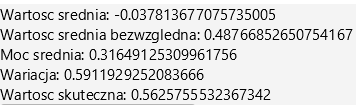
\includegraphics{cps_szum_o_rozkladzie_jednostajnym_wart.png}
    \caption{Wartości obliczone dla szumu o rozkładzie jednostajnym dla parametrów:  A=1, t1=0s, d=1s}
    \label{wartości dla eksperymentu 2}
\end{figure}
Wygenerowany szum widoczny na rysunku nr \ref{wykres dla eksperymentu 2} posiada rozkład jednostajny co obrazują wartości zawarte w histogramie z rysunku nr \ref{histogram dla eksperymentu 2}


%%%%%%%%%%%%%%%%%%%%%%%%%%%%%%%%%%%%%%%%%%%%%%%%%%%%%%%%%%%%%%%%%%%%%%%%%%%%%%%%%%%%%%%%%%%%%%%%%%%%%%%%%%%%%%%%%

%%%%%%%%%%%%%%%%%%%%%%%%%%%%%%%%%%%%%%%%%%%%%%%%%%%%%%%%%%%%%%%%%%%%%%%%%%%%%%%%%%%%%%%%%%%%%%%%%%%%%%%%%%%%%%%%%
\newpage
\subsection{Eksperyment nr 3: Impuls jednostkowy}

Eksperyment nr 3 polegał na wygenerowaniu impulsu jednostkowego. Impuls jednostkowy jest sygnałem dyskretnym który dla prawie wszystkich próbek przyjmuje wartości równe 0, jedynie dla jednej sprecyzowanej próbki przyjmuje wartość amplitudy.
\subsubsection{Założenia}
W eksperymencie impuls jednostkowy został wygenerowany dla następujących parametrów:
\begin{itemize}
    \item Amplituda 4
    \item Czas początkowy 1s
    \item Czas trwania 5s
    \item Częstotliwość 4 Hz
    \item Numer próbki, dla której następuje skok 12
\end{itemize}
\subsubsection{Przebieg}
Wygenerowany sygnał prezentuje się następująco:
\begin{figure}[H]
    \centering
    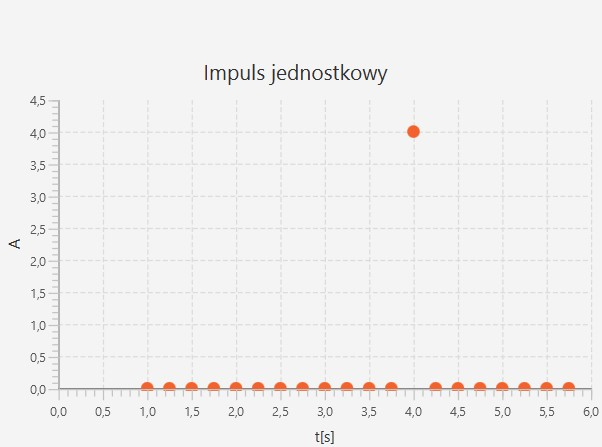
\includegraphics{cps_impuls_sygnal.jpg}
    \caption{Wykres impulsu jednostkowego dla parametrów:  A=1, t1=1s, d=5s, f=4Hz, ns=12}
    \label{wykres dla eksperymentu 3}
\end{figure}

Histogram dla powyższego impulsu wygląda następująco:
\begin{figure}[H]
    \centering
    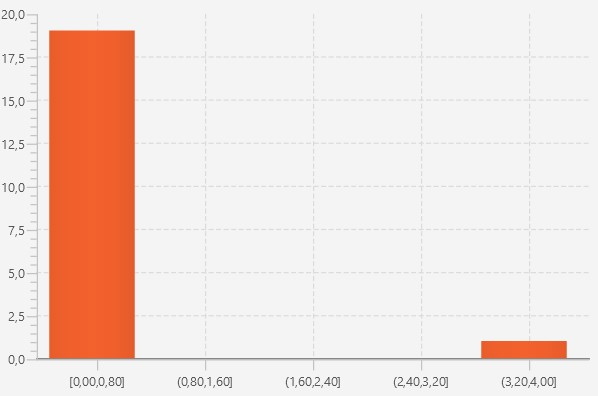
\includegraphics{cps_impuls_histogram.jpg}
    \caption{Histogram dla impulsu jednostkowego dla parametrów:  A=1, t1=1s, d=5s, f=4Hz, ns=12}
    \label{histogram dla eksperymentu 3}
\end{figure}


\subsubsection{Rezultat}
Obliczone parametry dla impulsu jednostkowego:
\begin{figure}[H]
    \centering
    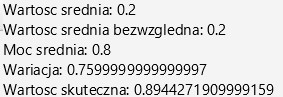
\includegraphics{cps_impuls_wartosci.jpg}
    \caption{Wartości obliczone dla impulsu jednostkowego dla parametrów:  A=1, t1=1s, d=5s, f=4Hz, ns=12}
    \label{wartości dla eksperymentu 3}
\end{figure}


%%%%%%%%%%%%%%%%%%%%%%%%%%%%%%%%%%%%%%%%%%%%%%%%%%%%%%%%%%%%%%%%%%%%%%%%%%%%%%%%%%%%%%%%%%%%%%%%%%%%%%%%%%%%%%%%%

%%%%%%%%%%%%%%%%%%%%%%%%%%%%%%%%%%%%%%%%%%%%%%%%%%%%%%%%%%%%%%%%%%%%%%%%%%%%%%%%%%%%%%%%%%%%%%%%%%%%%%%%%%%%%%%%%
\newpage
\subsection{Eksperyment nr 4: Dodawanie szumu gaussowskiego oraz sygnału sinusoidalnego}

Eksperyment nr 4 polegał na wygenerowaniu dwóch sygnałów (szumu gaussowskiego oraz sygnału sinusoidalnego) i dodaniu ich do siebie. Szum Gaussowski jest sygnałem którego amplituda przyjmuje losowe wartości z przedziału $<-A_{Gmax},A_{Gmax}>$ których rozkład prawdopodobieństwa jest rozkładem normalnym. Sygnał sinusoidalny opisuje funkcja:
\begin{equation}
    x(t)=Asin({2\PI}over{T}(t-t_1))
\end{equation}
\subsubsection{Założenia}
W eksperymencie szum został wygenerowany dla parametrów:
\begin{itemize}
    \item Amplituda: 0.1
    \item Czas początkowy: 0s
    \item Czas trwania sygnału: 2s
\end{itemize}
Sygnał sinusoidalny został wygenerowany dla parametrów:
\begin{itemize}
    \item Amplituda: 1
    \item Czas początkowy: 0s
    \item Czas trwania sygnału: 2s
    \item Okres: 1s
\end{itemize}
\subsubsection{Przebieg}

W trakcie tego eksperymentu jako składniki dodawania wygenerowane zostały sygnały których wykresy, histogramy oraz obliczone wartości zostały pokazane na rysunkach od \ref{wykres dla sinusa} do \ref{wartosci dla szumu gausowskiego}
\begin{figure}[H]
    \centering
    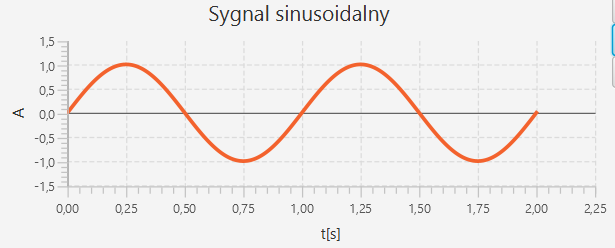
\includegraphics{cps_sinus_syg.PNG}
    \caption{Wykres sygnału sinusoidalnego dla parametrów:  A=1, t1=0s, d=1s, T=1s}
    \label{wykres dla sinusa}
\end{figure}
\begin{figure}[H]
    \centering
    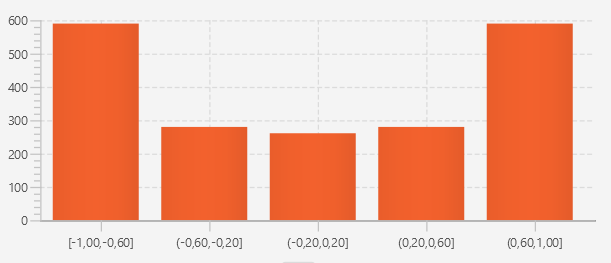
\includegraphics{cps_sinus_hist.PNG}
    \caption{Histogram sygnału sinusoidalnego dla parametrów:  A=1, t1=0s, d=1s, T=1s}
    \label{histogram dla sinusa}
\end{figure}
\begin{figure}[H]
    \centering
    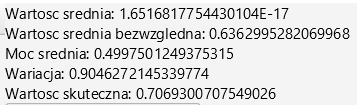
\includegraphics{cps_sinus_wart.PNG}
    \caption{Wartości obliczone dla sygnału sinusoidalnego dla parametrów:  A=1, t1=0s, d=1s, T=1s}
    \label{wartosci dla sinusa}
\end{figure}
\begin{figure}[H]
    \centering
    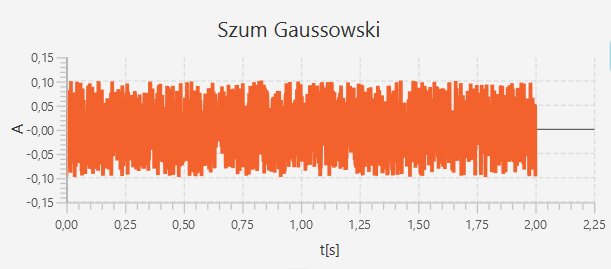
\includegraphics{cps_szum_gaussowski_syg.PNG}
    \caption{Wykres dla szumu gaussowskiego dla parametrów:  A=0.1, t1=0s, d=1s}
    \label{wykres dla szumu gausowskiego}
\end{figure}
\begin{figure}[H]
    \centering
    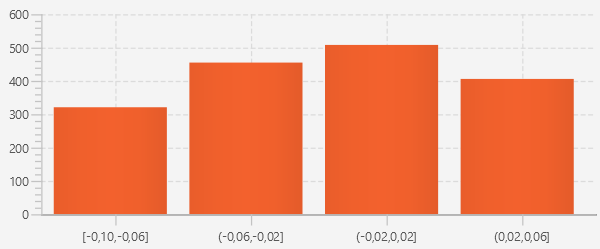
\includegraphics{cps_szum_gaussowski_hist.PNG}
    \caption{Histogram dla szumu gaussowskiego dla parametrów:  A=0.1, t1=0s, d=1s}
    \label{histogram dla szumu gausowskiego}
\end{figure}
\begin{figure}[H]
    \centering
    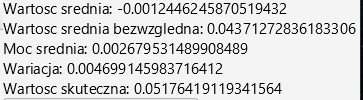
\includegraphics{cps_szum_gaussowski_wart.PNG}
    \caption{Wartości obliczone dla szumu gaussowskiego dla parametrów:  A=0.1, t1=0s, d=1s}
    \label{wartosci dla szumu gausowskiego}
\end{figure}

\subsubsection{Rezultat}
W wyniku dodania do siebie szumu gaussowskiego oraz sygnału sinusoidalnego otrzymaliśmy następujące wyniki:
\begin{figure}[H]
    \centering
    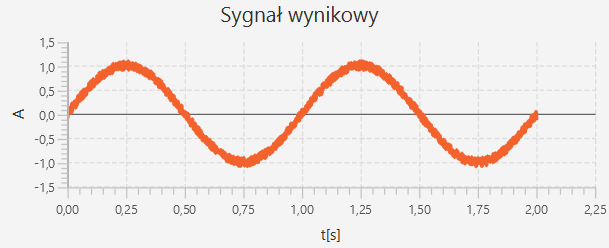
\includegraphics{cps_dodawanie_syg.PNG}
    \caption{Wartości obliczone dla sumy powyższych dwóch sygnałów}
    \label{wykres dodawania}
\end{figure}
\begin{figure}[H]
    \centering
    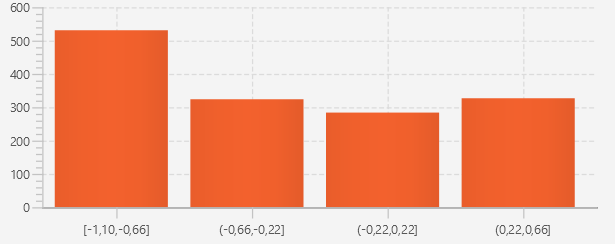
\includegraphics{cps_dodawanie_hist.PNG}
    \caption{Wartości obliczone dla sumy powyższych dwóch sygnałów}
    \label{histogram dodawania}
\end{figure}
\begin{figure}[H]
    \centering
    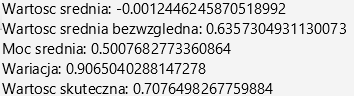
\includegraphics{cps_dodawanie_wart.PNG}
    \caption{Wartości obliczone dla sumy powyższych dwóch sygnałów}
    \label{wartosci dodawania}
\end{figure}


%%%%%%%%%%%%%%%%%%%%%%%%%%%%%%%%%%%%%%%%%%%%%%%%%%%%%%%%%%%%%%%%%%%%%%%%%%%%%%%%%%%%%%%%%%%%%%%%%%%%%%%%%%%%%%%%%

%%%%%%%%%%%%%%%%%%%%%%%%%%%%%%%%%%%%%%%%%%%%%%%%%%%%%%%%%%%%%%%%%%%%%%%%%%%%%%%%%%%%%%%%%%%%%%%%%%%%%%%%%%%%%%%%%
\newpage
\subsection{Eksperyment nr 5: Odejmowanie od sygnału sinusoidalnego wyprostowanego jednopołówkowo sygnału prostokątnego}
Eksperyment nr 5 polegał na wygenerowaniu dwóch sygnałów(sygnału sinusoidalnego wyprostowanego jednopołówkowo oraz sygnału prostokątnego) a następnie na obliczeniu różnicy tych sygnałów. Sygnał sinusoidalny wyprostowany jednopołówkowo posiada jedynie wartości nieujemne amplitudy i można opisać go funkcją:
\begin{equation}
    x(t)= 1 \over 2 A[sin({2\PI} \over {T} (t-t_1))+|sin({2\PI} \over {T} (t-t_1))|].
\end{equation}
Dla sygnału prostokątnego amplituda przyjmuje wartość zero lub $A_max$ i można go opisać wzorem:
\begin{equation}
    x(t)=\left\{\begin{matrix}A \: dla\: t\in \left \langle <kT+t_1, k_wT+kT+t_1)\right\\
    0 \: dla \: t\in \left \langle<k_wT-kT+t_1, T+kT+t_1\right\end{matrix} .\right
\end{equation}
\subsubsection{Założenia}
W eksperymencie sygnał sinusoidalny wyprostowany jednopołówkowo został wygenerowany dla parametrów:
\begin{itemize}
    \item Amplituda: 1
    \item Czas początkowy: 0s
    \item Czas trwania sygnału: 2s
    \item Okres: 1s
\end{itemize}
Sygnał prostokątny został wygenerowany dla parametrów:
\begin{itemize}
    \item Amplituda: 2
    \item Czas początkowy: 0s
    \item Czas trwania sygnału: 2s
    \item Okres: 1s
    \item Współczynnnik wypełnienia: 0.5
\end{itemize}
\subsubsection{Przebieg}
W trakcie tego eksperymentu wygenerowane zostały sygnały których wykresy, histogramy oraz obliczone wartości zostały pokazane na rysunkach od \ref{wykres dla sinusa jednopolowkowego} do \ref{wartosci dla prostokatnego}
\begin{figure}[H]
    \centering
    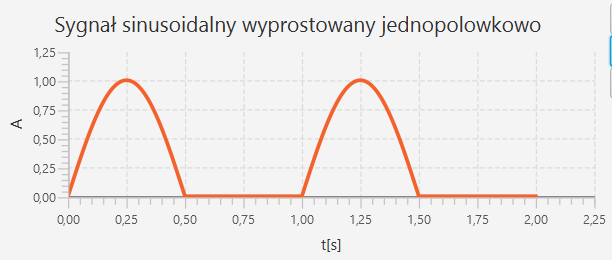
\includegraphics{cps_sinus_jednopolowkowy_syg.PNG}
    \caption{Wykres sygnału sinusoidalnego wyprostowanego jednopołówkowo dla parametrów:  A=1, t1=0s, d=2s, T=1s}
    \label{wykres dla sinusa jednopolowkowego}
\end{figure}
\begin{figure}[H]
    \centering
    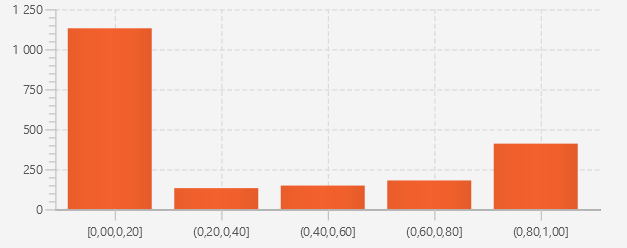
\includegraphics{cps_sinus_jednopolowkowy_hist.PNG}
    \caption{histogram sygnału sinusoidalnego wyprostowanego jednopołówkowo dla parametrów:  A=1, t1=0s, d=2s, T=1s}
    \label{histogram dla sinusa jednopolowkowego}
\end{figure}
\begin{figure}[H]
    \centering
    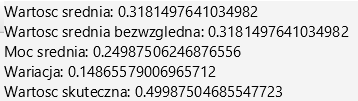
\includegraphics{cps_sinus_jednopolowkowy_wart.PNG}
    \caption{Wartości obliczone dla sygnału sinusoidalnego wyprostowanego jednopołówkowo dla parametrów:  A=1, t1=0s, d=2s, T=1s}
    \label{wartosci dla sinusa jednopolowkowego}
\end{figure}

\begin{figure}[H]
    \centering
    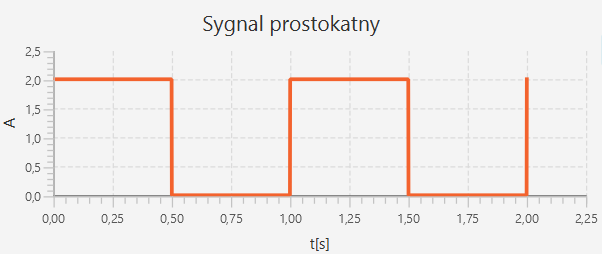
\includegraphics{cps_sygnal_prostokatny_syg.PNG}
    \caption{Wykres sygnału prostokątnego dla parametrów:  A=2, t1=0s, d=2s, T=1s, k_w=0.5}
    \label{wykres dla prostokatnego}
\end{figure}
\begin{figure}[H]
    \centering
    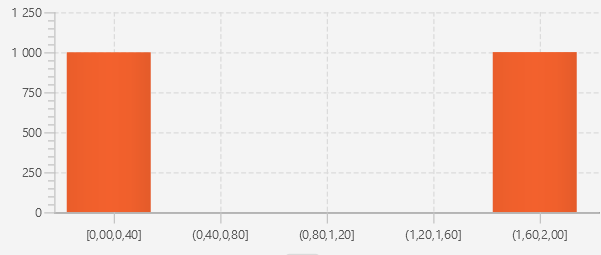
\includegraphics{cps_sygnal_prostokatny_hist.PNG}
    \caption{histogram sygnału prostokątnego dla parametrów:  A=2, t1=0s, d=2s, T=1s, k_w=0.5}
    \label{histogram dla prostokatnego}
\end{figure}
\begin{figure}[H]
    \centering
    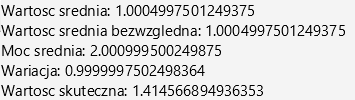
\includegraphics{cps_sygnal_prostokatny_wart.PNG}
    \caption{Wykres sygnału prostokątnego dla parametrów:  A=2, t1=0s, d=2s, T=1s, k_w=0.5}
    \label{wartosci dla prostokatnego}
\end{figure}
\subsubsection{Rezultat}
W wyniku odjęcia od sygnału sinusoidalnego wyprostowanego jednopołówkowo sygnału prostokątnego otrzymaliśmy widoczne poniżej wyniki.
\begin{figure}[H]
    \centering
    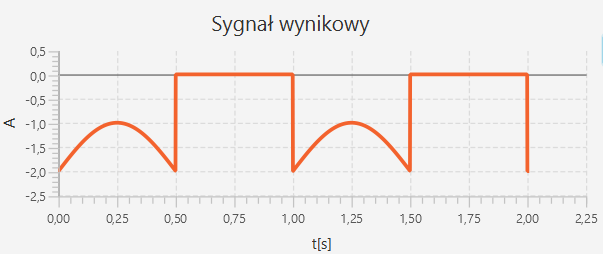
\includegraphics{cps_odejmowanie_syg.PNG}
    \caption{Wykres sygnału wynikowego operacji odejmowania}
    \label{wykres dla odejmowania}
\end{figure}
\begin{figure}[H]
    \centering
    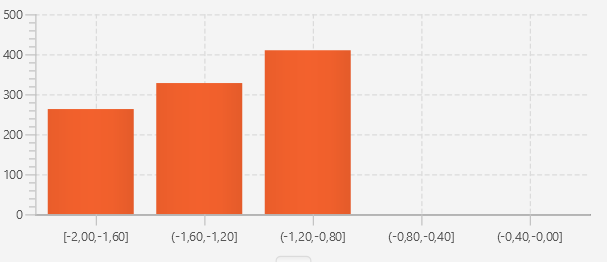
\includegraphics{cps_odejmowanie_hist.PNG}
    \caption{Histogram sygnału wynikowego operacji odejmowania}
    \label{histogram dla odejmowania}
\end{figure}
\begin{figure}[H]
    \centering
    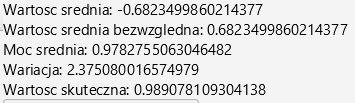
\includegraphics{cps_odejmowanie_wart.PNG}
    \caption{Wartości obliczone dla sygnału wynikowego operacji odejmowania}
    \label{wartosci dla odejmowania}
\end{figure}


%%%%%%%%%%%%%%%%%%%%%%%%%%%%%%%%%%%%%%%%%%%%%%%%%%%%%%%%%%%%%%%%%%%%%%%%%%%%%%%%%%%%%%%%%%%%%%%%%%%%%%%%%%%%%%%%%

%%%%%%%%%%%%%%%%%%%%%%%%%%%%%%%%%%%%%%%%%%%%%%%%%%%%%%%%%%%%%%%%%%%%%%%%%%%%%%%%%%%%%%%%%%%%%%%%%%%%%%%%%%%%%%%%%
\newpage
\subsection{Eksperyment nr 6: Mnożenie sygnału sinusoidalnego wyprostowanego dwupołówkowo oraz sygnału symetrycznego prostokątnego}
Eksperyment nr 6 polegał na pomnożeniu przez siebie sygnału sinusoidalnego wyprostowanego dwupołówkowo z sygnałem symetrycznym prostokątnego, w wyniku czego otrzymany został sygnał wynikowy.\\
Funkcja opisująca sygnał sinusoidalny wyprostowany dwupołówkowo wygląda tak:
\begin{equation}
    x(t) = A\left | sin(\frac{2\pi}{T}(t-t_1)) \right |
\end{equation}
Natomiast funkcja opisująca sygnał prostokątny symetryczny prezentuje się następująco:
\begin{equation}
    x(t) = \left\{\begin{matrix} A \: dla \: t\in \left \langle kT+t_1,k_wT+kT+t_1 \right )\\ -A \: dla \: t \in \left \langle k_2T+t_1+kT,T+kT+t_1 \right) \end{matrix}\right. dla \: k\in C\
\end{equation}


\subsubsection{Założenia}
W eksperymencie sygnały zostały wygenerowane dla następujących parametrów:
\\
Dla sygnału sinusoidalnego wyprostowanego dwupołówkowo:
\begin{itemize}
    \item Amplituda = 1
    \item Czas początkowy = 2s
    \item Czas trwania sygnału = 5s
    \item Okres podstawowy = 3s
\end{itemize}
Dla sygnału prostokątnego symetrycznego:
\begin{itemize}
    \item Amplituda = 2
    \item Czas początkowy = 3s
    \item Czas trwania sygnału = 6s
    \item Okres podstawowy = 2s
    \item Współczynnik wypełnienia = 0.43
\end{itemize}
\subsubsection{Przebieg}
Wygenerowany wykres sygnału sinusoidalnego wyprostowanego dwupołówkowo wygląda następująco:
\begin{figure}[H]
    \centering
    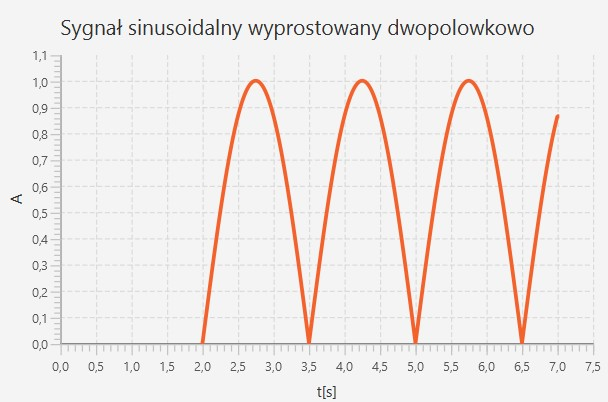
\includegraphics{cps_sin_dwupolowkowy_sygnal.jpg}
    \caption{Wykres sygnału sinusoidalnego wyprostowanego dwupołówkowo dla parametrów:  A=1, t1=2s, d=5s, T=3s.}
    \label{Wykres dla sygnału sinusoidalnego dwupołówkowego}
\end{figure}

Histogram dla powyższego wykresu prezentuje się następująco:
\begin{figure}[H]
    \centering
    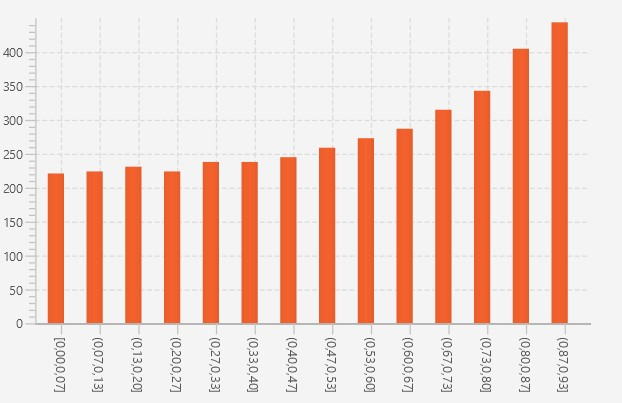
\includegraphics{cps_sin_dwupolowkowy_histogram.jpg}
    \caption{Histogram dla sygnału sinusoidalnego wyprostowanego dwupołówkowo dla parametrów:  A=1, t1=2s, d=5s, T=3s.}
    \label{Histogram dla sygnału sinusoidalnego dwupołówkowego}
\end{figure}

Natomiast obliczone wartości dla sygnału sinusoidalnego wyprostowanego dwupołówkowo są następujące:
\begin{figure}[H]
    \centering
    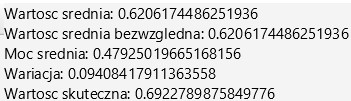
\includegraphics{cps_sin_dwupolowkowy_wartosci.jpg}
    \caption{Wartości obliczone dla sygnału sinusoidalnego wyprostowanego dwupołówkowo dla parametrów:  A=1, t1=2s, d=5s, T=3s.}
    \label{Wartości dla sygnału sinusoidalnego dwupołówkowego}
\end{figure}

Dla drugiego sygnału, czyli sygnału protokątnego symetrycznego został uzyskany następujący wykres:
\begin{figure}[H]
    \centering
    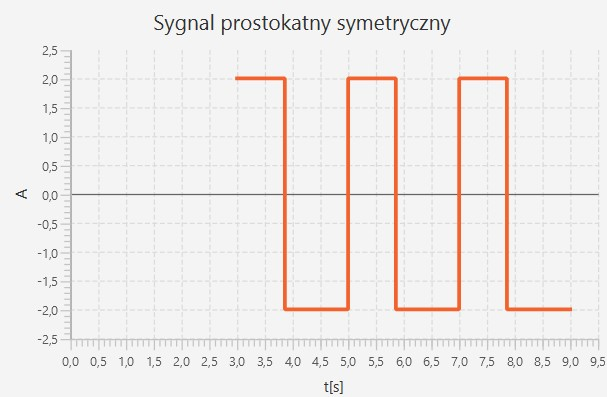
\includegraphics{cps_prost_symetryczny_sygnal.jpg}
    \caption{Wykres sygnału prostokątnego symetrycznego dla parametrów:  A=2, t1=3s, d=6s, T=2s, k=0.43.}
    \label{Histogram dla sygnału prostokątnego symetrycznego}
\end{figure}

Histogram dla powyższego wykresu wygląda następująco:
\begin{figure}[H]
    \centering
    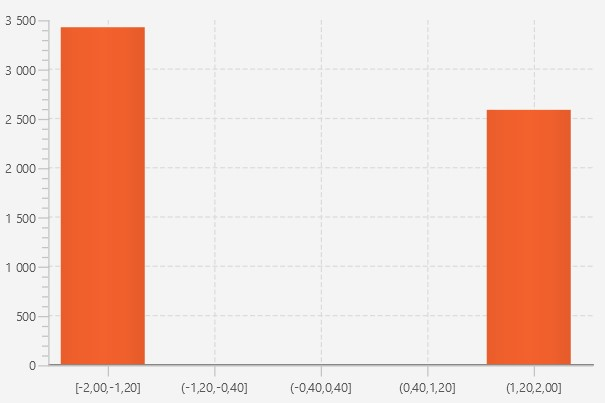
\includegraphics{cps_prost_symetryczny_histogram.jpg}
    \caption{Histogram dla sygnału prostokątnego symetrycznego dla parametrów:  A=2, t1=3s, d=6s, T=2s, k=0.43.}
    \label{Wykres dla sygnału prostokątnego symetrycznego}
\end{figure}

Obliczone wartości dla sygnału prostokątnego symetrycznego prezentują się następująco:
\begin{figure}[H]
    \centering
    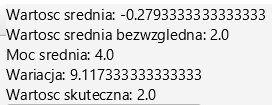
\includegraphics{cps_prost_symetryczny_wartosci.jpg}
    \caption{Wartości obliczone dla sygnału prostokątnego symetrycznego dla parametrów:  A=2, t1=3s, d=6s, T=2s, k=0.43.}
    \label{Wartości dla sygnału prostokątnego symetrycznego}
\end{figure}
\subsubsection{Rezultat}
W wyniku przeprowadzonego eksperymentu powstał następujący sygnał wynikowy:
\begin{figure}[H]
    \centering
    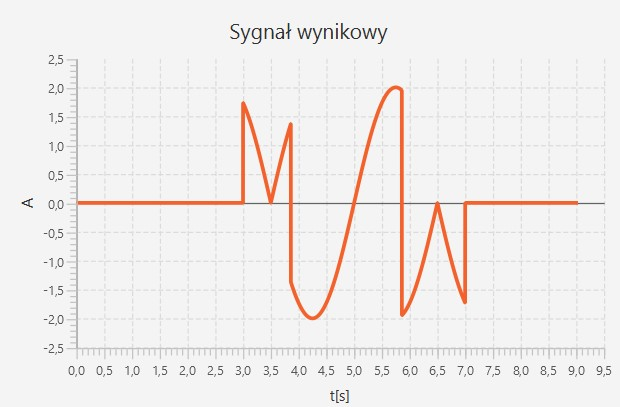
\includegraphics{cps_mnozenie_wykres.jpg}
    \caption{Wykres sygnału będącego wynikiem mnożenia sygnału sinusoidalnego wyprostowanego dwupółkowo i sygnału prostokątnego symetrycznego.}
    \label{Wykres dla mnożenia}
\end{figure}

Histogram dla powyższego wykresu wygląda tak:
\begin{figure}[H]
    \centering
    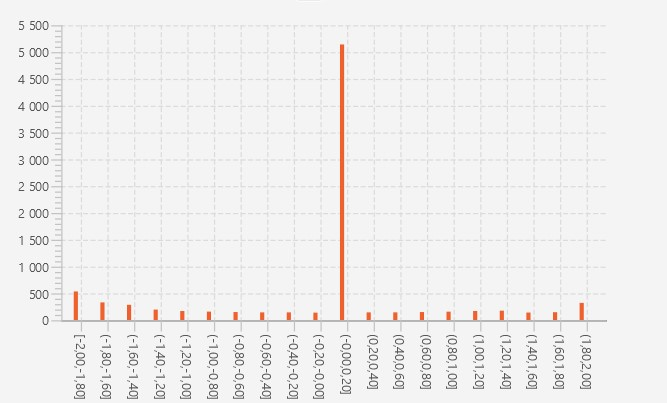
\includegraphics{cps_mnozenie_histogram.jpg}
    \caption{Histogram dla sygnału będącego wynikiem mnożenia sygnału sinusoidalnego wyprostowanego dwupółkowo i sygnału prostokątnego symetrycznego.}
    \label{Histogram dla mnożenia}
\end{figure}

Natomiast obliczone wartości prezentują się w następujący sposób:
\begin{figure}[H]
    \centering
    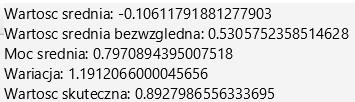
\includegraphics{cps_mnozenie_wartosci.jpg}
    \caption{Wartości obliczone sygnału będącego wynikiem mnożenia sygnału sinusoidalnego wyprostowanego dwupółkowo i sygnału prostokątnego symetrycznego.}
    \label{Wartości dla mnożenia}
\end{figure}


%%%%%%%%%%%%%%%%%%%%%%%%%%%%%%%%%%%%%%%%%%%%%%%%%%%%%%%%%%%%%%%%%%%%%%%%%%%%%%%%%%%%%%%%%%%%%%%%%%%%%%%%%%%%%%%%%

%%%%%%%%%%%%%%%%%%%%%%%%%%%%%%%%%%%%%%%%%%%%%%%%%%%%%%%%%%%%%%%%%%%%%%%%%%%%%%%%%%%%%%%%%%%%%%%%%%%%%%%%%%%%%%%%%
\newpage
\subsection{Eksperyment nr 7: Dzielenie sygnału trójkątnego przez skok jednostkowy}
Celem eksperymentu nr 7 było wygenerowanie sygnału będącego wynikiem dzielenia sygnału trójkątnego przez skok jednostkowy.
Funkcja opisująca sygnał trójkątny prezentuje się następująco:
 \begin{equation}
    x(t) = \left\{\begin{matrix} \frac{A}{k_wT}(t-kT-t_1)\: dla \: t\in \left \langle kT + t_1,k_wT + kT + t_1 \right) \\ \frac{-A}{T(1-k_w)}(t - kT - t_1) + \frac{A}{1-k_w}\: dla \: t\in \left \langle k_wT + t_1 + kT, T + kT + t_1 \right) \end{matrix}\right. dla \: k\in C\    
 \end{equation}
Natomiast funkcja opisująca skok jednostkowy wygląda następująco:
\begin{equation}
    x(t) = \left\{\begin{matrix} A \: dla \: t>t_s \\ \frac{1}{2} \: dla \: t=t_s \\ 0 \: dla \: t<t_s \end{matrix}\right.\    
\end{equation}



\subsubsection{Założenia}
W eksperymencie sygnały zostały wygenerowane dla następujących parametrów:\\
Dla sygnału trójkątnego:
\begin{itemize}
    \item Amplituda = 5
    \item Czas początkowy = 0s
    \item Czas trwania sygnału = 4s
    \item Okres podstawowy = 1s
    \item Współczynnik wypełnienia = 0.2
\end{itemize}

Dla skoku jednostkowego:
\begin{itemize}
    \item Amplituda = 4
    \item Czas początkowy = 0s
    \item Czas trwania sygnału = 4s
    \item Czas skoku = 3s
\end{itemize}


\subsubsection{Przebieg}
Wygenerowany sygnał trójkątny prezentuje się następująco:
\begin{figure}[H]
    \centering
    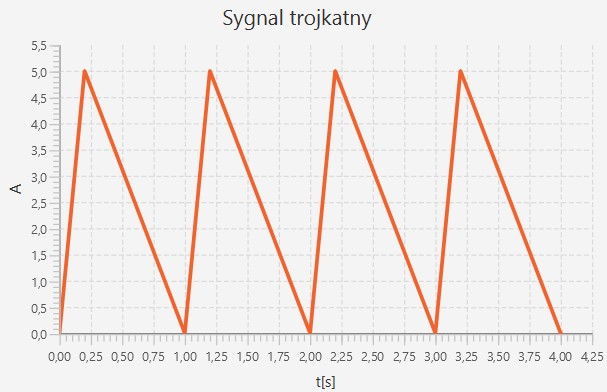
\includegraphics{cps_trojkatny_sygnal.jpg}
    \caption{Wykres sygnału trójkątnego dla parametrów:  A=5, t1=0s, d=4s, T=1s, k=0.2.}
    \label{Wykres dla sygnału trójkątnego}
\end{figure}

Histogram dla powyższego sygnału trójkątnego ma postać:
\begin{figure}[H]
    \centering
    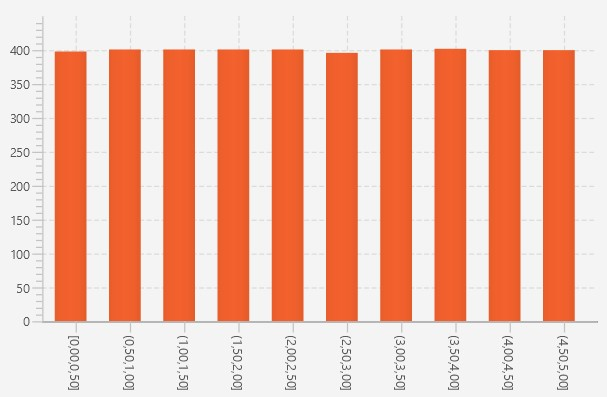
\includegraphics{cps_trojkatny_histogram.jpg}
    \caption{Histogram dla sygnału trójkątnego dla parametrów:  A=5, t1=0s, d=4s, T=1s, k=0.2.}
    \label{histogram dla sygnału trójkątnego}
\end{figure}

Natomiast obliczone wartości dla sygnału trójkątnego są następujące:
\begin{figure}[H]
    \centering
    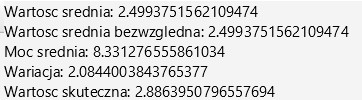
\includegraphics{cps_trojkatny_wartosci.jpg}
    \caption{Wartości obliczone dla sygnału trójkątnego dla parametrów:  A=5, t1=0s, d=4s, T=1s, k=0.2.}
    \label{Wartości dla sygnalu trójkątnego}
\end{figure}


Dla skoku jednostkowego, przez który dzieliliśmy sygnał trójkątny wykres wygląda następująco:
\begin{figure}[H]
    \centering
    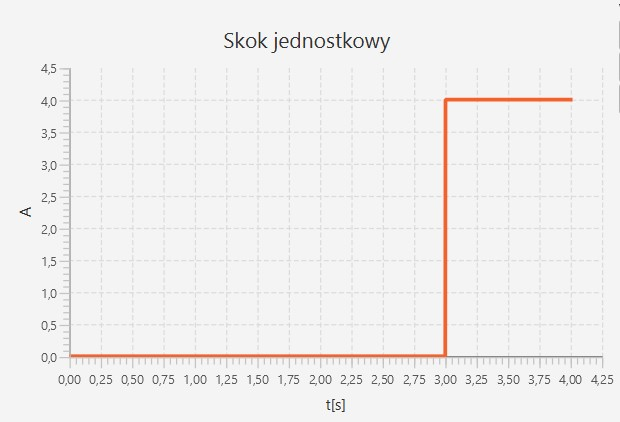
\includegraphics{cps_jednostkowy_sygnal.jpg}
    \caption{Wykres skoku jednostkowego dla parametrów:  A=4, t1=0s, d=4s, ts=3s.}
    \label{wykres dla skoku jednostkowego}
\end{figure}

Histogram dla powyższego wykresu skoku jednostkowego ma postać:
\begin{figure}[H]
    \centering
    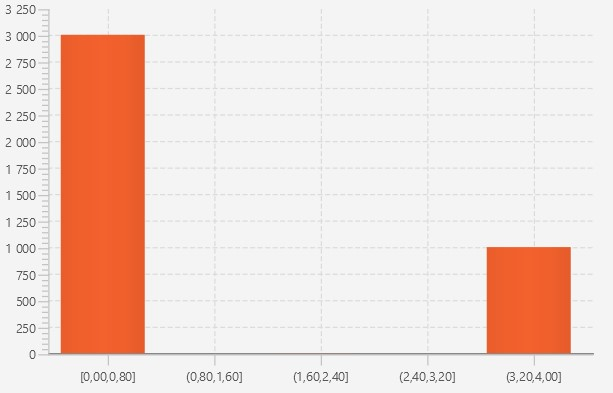
\includegraphics{cps_jednostkowy_histogram.jpg}
    \caption{Histogram dla jednostkowego dla parametrów:  A=4, t1=0s, d=4s, ts=3s.}
    \label{histogram dla skoku jednostkowego}
\end{figure}

Obliczone wartości dla skoku jednostkowego są następujące:
\begin{figure}[H]
    \centering
    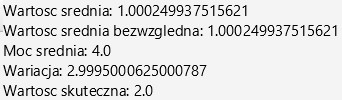
\includegraphics{cps_jednostkowy_wartosci.jpg}
    \caption{Wartości obliczone dla skoku jednostkowego dla parametrów:  A=4, t1=0s, d=4s, ts=3s.}
    \label{wartości dla skoku jednostkowego}
\end{figure}
\subsubsection{Rezultat}
W wyniku przeprowadzonego eksperymentu powstał sygnał wynikowy, który wygląda następująco:
\begin{figure}[H]
    \centering
    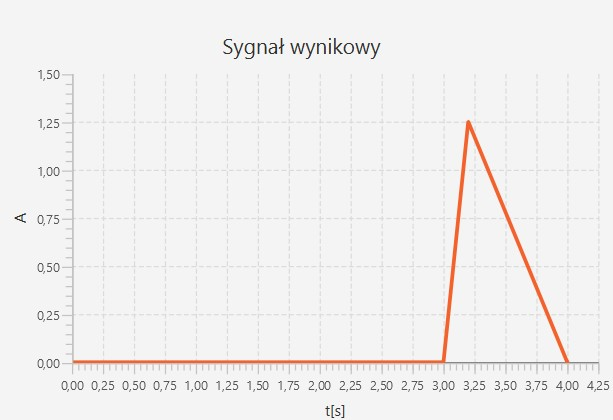
\includegraphics{cps_dzielenie_sygnal.jpg}
    \caption{Wykres sygnału, będącego wynikiem dzielenia sygnału trójkątnego przez skok jednostkowy.}
    \label{wykres dla dzielenia}
\end{figure}

Histogram dla powyższego sygnału wynikowego wygląda tak:
\begin{figure}[H]
    \centering
    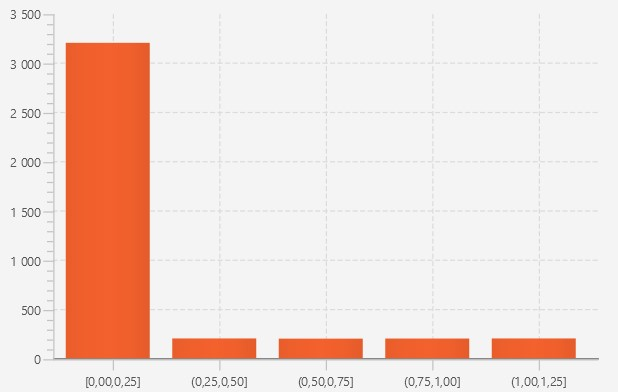
\includegraphics{cps_dzielenie_histogram.jpg}
    \caption{Histogram dla sygnału, będącego wynikiem dzielenia sygnału trójkątnego przez skok jednostkowy.}
    \label{histogram dla dzielenia}
\end{figure}

Natomiast wartości, jakie otrzymaliśmy w ramach tej operacji prezentują się następująco:
\begin{figure}[H]
    \centering
    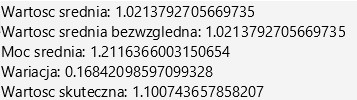
\includegraphics{cps_dzielenie_wartosci.jpg}
    \caption{Wartości obliczone dla dzielenia sygnału trójkątnego przez skok jednostkowy.}
    \label{wartości dla dzielenia}
\end{figure}


%%%%%%%%%%%%%%%%%%%%%%%%%%%%%%%%%%%%%%%%%%%%%%%%%%%%%%%%%%%%%%%%%%%%%%%%%%%%%%%%%%%%%%%%%%%%%%%%%%%%%%%%%%%%%%%%%

%%%%%%%%%%%%%%%%%%%%%%%%%%%%%%%%%%%%%%%%%%%%%%%%%%%%%%%%%%%%%%%%%%%%%%%%%%%%%%%%%%%%%%%%%%%%%%%%%%%%%%%%%%%%%%%%%

\section{Wnioski}
\begin{itemize}
    \item Każdy sygnał ciągły można zdyskretyzować poprzez próbkowanie.
    \item Program poprawnie generuje zaimplementowane sygnały.
    \item Program pozwala na proste działania na sygnałach.
    \item Na podstawie histogramów w prosty sposób można dowiedzieć się o rozkładzie wartości.
\end{itemize}
 

%%%%%%%%%%%%%%%%%%%%%%%%%%%%%%%%%%%%%%%%%%%%%%%%%%%%%%%%%%%%%%%%%%%%%%%%%%%%%%%%%%%%%%%%%%%%%%%%%%%%%%%%%%%%%%%%%
% BIBLIOGRAFIA
%%%%%%%%%%%%%%%%%%%%%%%%%%%%%%%%%%%%%%%%%%%%%%%%%%%%%%%%%%%%%%%%%%%%%%%%%%%%%%%%%%%%%%%%%%%%%%%%%%%%%%%%%%%%%%%%%

\renewcommand\refname{Bibliografia}
\bibliographystyle{plain}
\bibliography{bibliografia_wzor}

\end{document}
